\documentclass[aspectratio=169]{beamer}
\usepackage{tikz}
\usepackage{listings}
\mode<presentation>

\title{digital plumbing}

\begin{document}
\begin{frame}
    \titlepage
\end{frame}

\begin{frame}{who am I?}
    \begin{description}[align=right]
        \setlength{\itemsep}{1cm}
        \item[undergrad:]
            \begin{itemize}
                \item BSc, Biomedical Engineering
                \item synthetic genomics/biology research advised by Jef Boeke
            \end{itemize}
        \item[currently:]
            \begin{itemize}
                \item PhD candidate, Biomedical Engineering
                \item research advised by Fred Winston
            \end{itemize}
    \end{description}
\end{frame}

\begin{frame}{grad school timeline}
\includegraphics[width=\textwidth]{figures/presentation_figure1-timeline.pdf}
\end{frame}

\begin{frame}{purpose of this meeting}
\end{frame}

\begin{frame}{I develop analysis pipelines for genomics data}
\end{frame}

\begin{frame}{genomics data and its analysis are complex}
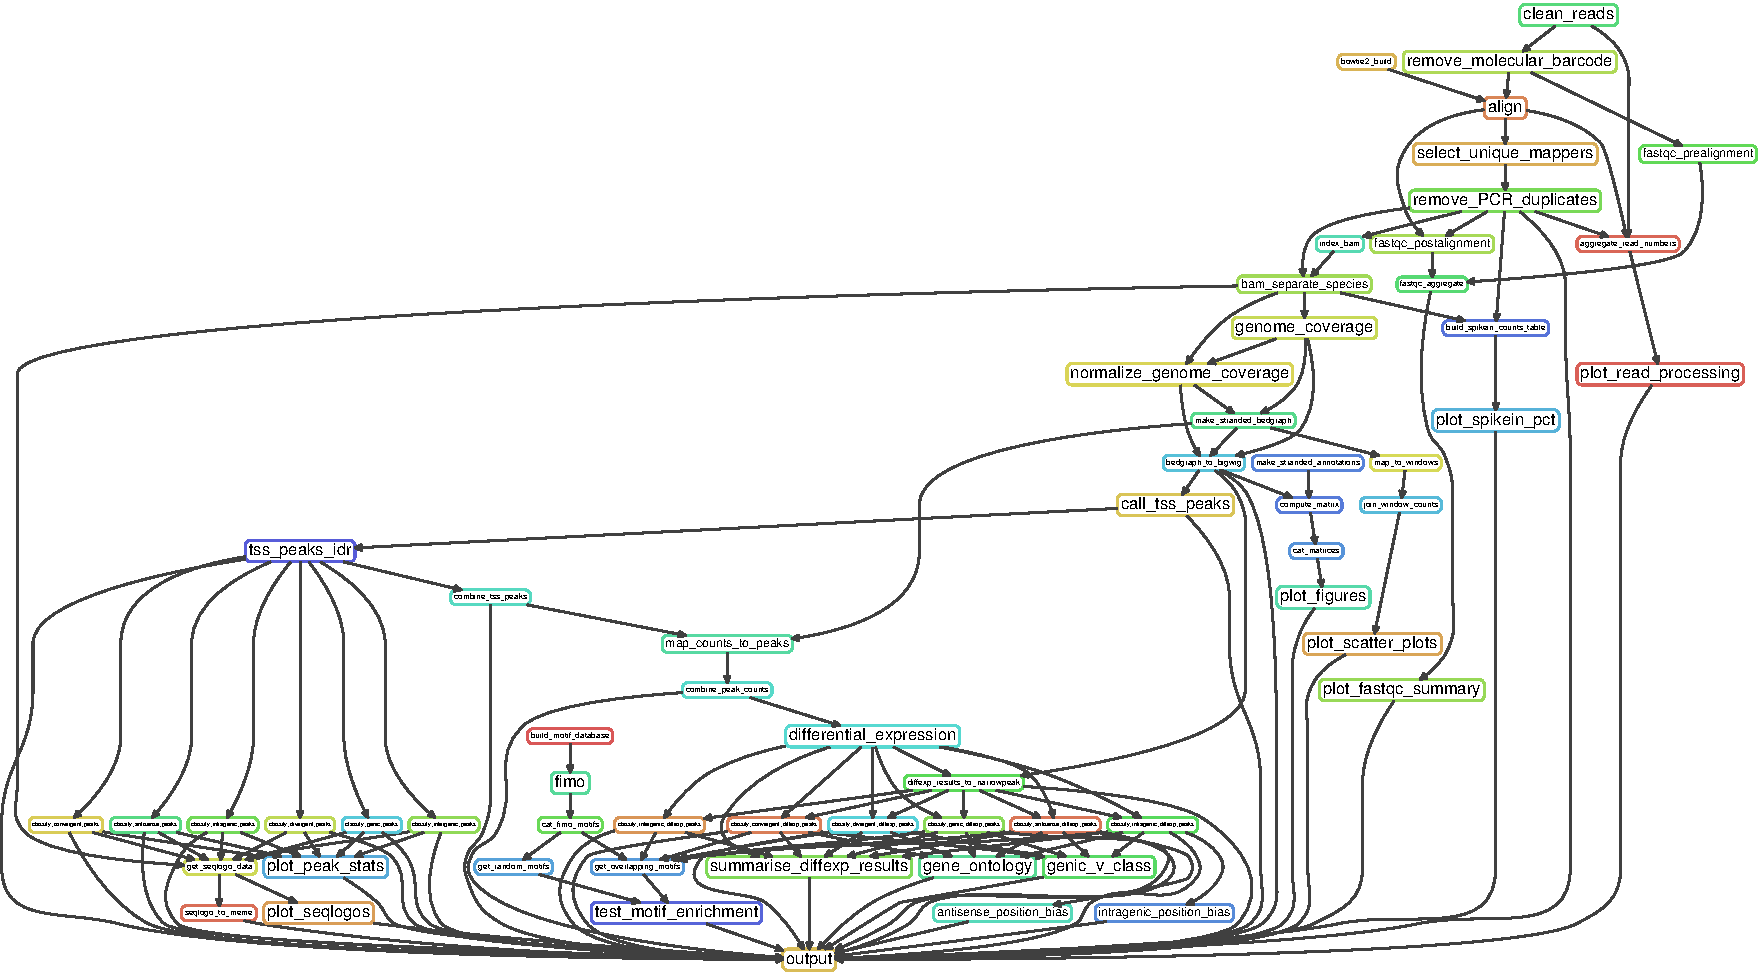
\includegraphics[width=\textwidth]{figures/rulegraph.pdf}
\end{frame}

\begin{frame}[fragile]{Snakemake for reproducible data analyses}
    \begin{itemize}
        \item a Python-based workflow management system developed by Johannes Köster
        \item \textbf{rules} describe how to create \textbf{output files} from \textbf{input files}:
            \begin{lstlisting}
            rule foobar:
                input: "input.txt"
                output: "output.txt"
                script: "turn_input_into_output.py"
            \end{lstlisting}
        \item dependency management using \textbf{conda}
        \item scalable from workstations to computing clusters
    \end{itemize}
\end{frame}

\begin{frame}{projects I'm working on}
    \begin{itemize}[]
        \setlength{\itemsep}{1cm}
        \item transcription elongation factor \textbf{Spt6}
        \item intragenic transcription in stress
        \item transcription elongation factor \textbf{Spt5}
    \end{itemize}
\end{frame}

\begin{frame}{intro to Spt6}
\end{frame}

\begin{frame}{Spt6 project collaborators}
    \begin{description}[align=right, noitemsep]
        \item [Steve Doris] optimized TSS-seq and ChIP-nexus protocols
        \item [] generated TSS-seq and ChIP-nexus libraries
        \item [Olga Viktorovskaya] generated MNase-seq libraries
        \item [Magdalenda Murawska] generated NET-seq libraries
        \item [Dan Spatt] wetlab experiments for publication
    \end{description}
\end{frame}

\begin{frame}{WASSDA}
\includegraphics[width=\textwidth]{figures/figure0_txn-diagram.pdf}
\end{frame}

% \begin{frame}
% \includegraphics[width=\textwidth]{figures/figure1_tss-seq-coverage.pdf}
% \end{frame}

% \begin{frame}
% \includegraphics[width=\textwidth]{figures/figure3_tfiib-nexus-tata.pdf}
% \end{frame}

\begin{frame}
    \begin{tikzpicture}
        \node<1,2>[anchor=south west, inner sep=0] at (0,0) {\includegraphics[width=\textwidth]{figures/presentation_figure0-mvd1-coverage.pdf}};
        \fill<1>[white] (0,0) rectangle (\textwidth, 4.38cm);
        \fill<2>[white, opacity=0] (0,0) rectangle (\textwidth, 4.38cm);
    \end{tikzpicture}
\end{frame}

\begin{frame}
    \begin{tikzpicture}
        \node<1,2>[anchor=south west, inner sep=0] at (0,0) {\includegraphics[width=\textwidth]{figures/presentation_figure2_tss-seq-heatmaps.pdf}};
        \draw<1>[ultra thick, draw=white, fill=white] (0.52\textwidth,0) rectangle (\textwidth, 8cm);
        \draw<2>[ultra thick, draw opacity=0] (0.52\textwidth,0) rectangle (\textwidth, 8cm);
    \end{tikzpicture}
\end{frame}

\begin{frame}
    \centering
    \includegraphics[height=0.2\textheight]{figures/figure0_txn-diagram.pdf}
    \begin{columns}
        \begin{column}{0.5\textwidth}
            \centering
            \includegraphics[width=\textwidth]{figures/presentation_figure6-tss-diffexp-summary.pdf}
        \end{column}
        \begin{column}{0.5\textwidth}
            \centering
            \pause
            \includegraphics[width=\textwidth]{figures/presentation_figure7-tss-expression-levels.pdf}
        \end{column}
    \end{columns}
\end{frame}

\begin{frame}
    \centering
    \includegraphics[width=12cm]{figures/presentation_figure3_tfiib-heatmaps.pdf}
\end{frame}

\begin{frame}{TFIIB is spread across the genome in \textit{spt6-1004}}
\includegraphics[width=\textwidth]{figures/presentation_figure14-tfiib-spreading-ssa4.pdf}
\end{frame}

\begin{frame}{new initiation contributes to most \textit{spt6-1004} intragenic transcripts}
    \centering
    \includegraphics[height=0.2\textheight]{figures/figure0_txn-diagram.pdf}
    \includegraphics[width=\textwidth]{figures/presentation_figure4_tss-v-tfiib.pdf}
\end{frame}

\begin{frame}{chromatin structure in \textit{spt6-1004}}
\includegraphics[width=\textwidth]{figures/presentation_figure9-mnase-metagene.pdf}
\end{frame}

\begin{frame}{quantifying changes in nucleosomes}
    \begin{columns}
        \begin{column}{0.5\textwidth}
            \centering
            \includegraphics[width=\textwidth]{figures/presentation_figure5-nucattributes.pdf}
        \end{column}
        \begin{column}{0.5\textwidth}
            \centering
            \pause
            \includegraphics[width=\textwidth]{figures/presentation_figure8-global-nuc-fuzz-occ.pdf}
        \end{column}
    \end{columns}
\end{frame}

\begin{frame}
\includegraphics[width=\textwidth]{figures/presentation_figure10-mnase-heatmaps.pdf}
\end{frame}

\begin{frame}
\includegraphics[width=\textwidth]{figures/presentation_figure11-intragenic-mnase.pdf}
\end{frame}

\begin{frame}{intragenic promoters share features with genic promoters}
    \includegraphics[width=\textwidth]{figures/presentation_figure12-seqlogos.pdf}
\end{frame}

\begin{frame}{intragenic promoters share features with genic promoters}
    \includegraphics[width=\textwidth]{figures/presentation_figure13-intragenic-tata.pdf}
\end{frame}

\begin{frame}{summary of Spt6 results}
    \begin{itemize}
        \item TSS-seq identifies over 8000 intragenic or antisense TSSs in \textit{spt6-1004}
        \item TFIIB is spread across the genome in \textit{spt6-1004}
        \item chromatin structure is severly disrupted in \textit{spt6-1004}
        \item \textit{spt6-1004} intragenic promoter share some features with genic promoters
    \end{itemize}
\end{frame}

\begin{frame}{software written}
    \begin{columns}
        \begin{column}{0.5\textwidth}
            \begin{itemize}
                \item TSS-seq
                \item ChIP-nexus
                \item MNase-seq
                \item NET- and RNA-seq
                \item integrated data visualization
                \item genome annotation
                \item motif enrichment
                \item assay correlations
                \item paired-end demultiplexing
                \item one-off data analyses
            \end{itemize}
        \end{column}
        \begin{column}{0.5\textwidth}
            \hspace{2.7em} 
\includegraphics[height=1.5em]{figures/github-small.pdf} \href{https://github.com/winston-lab}{github.com/winston-lab} \\
            \vspace{1em}
            
\includegraphics[height=1.5em]{figures/zenodo-black.pdf} \href{https://doi.org/10.5281/zenodo.1409826}{DOI: 10.5281/zenodo.1409826}
        \end{column}
    \end{columns}
    \begin{itemize}
        \item \small TSS-seq vs. TFIIB ChIP-nexus
        \item \small previous TSS-seq data (Malabat and Feuerbach \textit{et al}., 2015)
        \item \small ChIP-exo data (Rhee and Pugh, 2012)
        \item \small previous \textit{spt6-1004} data (Cheung \textit{et al}., 2008; Uwimana \textit{et al}., 2017)
        \item \small figure generation for publication
    \end{itemize}
\end{frame}

\begin{frame}{intragenic transcription in wild-type cells}
\end{frame}

\begin{frame}{collaborators}
    \begin{description}[align=right, noitemsep]
        \item [Steve Doris] generated TSS-seq and ChIP-nexus libraries
        \item [Dan Spatt] polyribosome fractionation
    \end{description}
\end{frame}

\begin{frame}
    TFIIB ChIP-nexus in three stress conditions:
    \begin{itemize}
        \item oxidative stress (diamide)
        \item amino acid starvation
        \item nitrogen starvation
    \end{itemize}
\end{frame}

\begin{frame}
\includegraphics[width=\textwidth]{figures/presentation_figure15-tfiib-heatmaps.pdf}
\end{frame}

\begin{frame}
    oxidative stress TSS-seq in three \textit{Saccharomyces} species:
    \begin{itemize}
        \item \textit{S. cerevisiae}
        \item \textit{S. mikatae}
        \item \textit{S. bayanus} var. \textit{uvarum}
    \end{itemize}
\end{frame}

\begin{frame}
    \begin{enumerate}
        \item induce oxidative stress
        \item get RNA associated with the polyribosome fraction
        \item prepare TSS-seq libraries
    \end{enumerate}
\end{frame}

\begin{frame}
    TODO
\end{frame}

\begin{frame}{Spt5}
    \begin{description}[align=right, noitemsep]
        \item [Ameet Shetty] generated TSS-seq, MNase-seq, NET-seq, RNA-seq, and ChIP-seq libraries
    \end{description}
\end{frame}

\begin{frame}{RNAPII accumulates at the 5' end of genes in Spt5 depletion}
    \includegraphics[width=\textwidth]{figures/presentation_figure16-netseq-metagene.pdf}
\end{frame}

\begin{frame}{antisense transcripts appear at the 5' ends of genes in Spt5 depletion}
    \includegraphics[width=\textwidth]{figures/presentation_figure17-rnaseq-heatmaps.pdf}
\end{frame}

\begin{frame}
    two more assays:
    \begin{itemize}
        \item TSS-seq
        \item MNase-seq
    \end{itemize}
\end{frame}

\begin{frame}
    \includegraphics[width=\textwidth]{figures/presentation_figure18-antisense-heatmaps.pdf}
\end{frame}

\begin{frame}{chromatin structure in Spt5 depletion}
    \includegraphics[width=\textwidth]{figures/presentation_figure19-mnase-metagene.pdf}
\end{frame}

\begin{frame}{chromatin structure at Spt5-depletion antisense TSSs}
    \includegraphics[width=\textwidth]{figures/presentation_figure20-antisense-mnase-metagene.pdf}
\end{frame}

\begin{frame}
    TODO
\end{frame}

\begin{frame}
    overall summary
\end{frame}

\begin{frame}{acknowledgements}
    \begin{columns}
        \begin{column}{0.5\textwidth}
            \begin{itemize}
                \item Winston lab
                    \begin{itemize}
                        \item Fred Winston
                        \item Ameet Shetty
                        \item Steve Doris
                        \item Olga Viktorovskaya
                        \item Magdalena Murawska
                        \item Dan Spatt
                        \item Natalia Reim
                        \item Rajaraman Gopalakrishnan
                        \item Francheska Lopez Rivera
                        \item Katie Weiner
                        \item James Warner
                        \item Mallory Rice
                    \end{itemize}
            \end{itemize}
        \end{column}
        \begin{column}{0.5\textwidth}
            \begin{itemize}
                \item committee
                    \begin{itemize}
                        \item Fred Winston
                        \item Mo Khalil
                        \item Stirling Churchman
                        \item John Ngo
                        \item Daniel Segre
                    \end{itemize}
                \item HMS Research Computing
            \end{itemize}
            \begin{description}
                \item [\href{https://github.com/winston-lab}{github.com/winston-lab}]
                \item [\href{https://github.com/james-chuang}{github.com/james-chuang}]
                \item [\href{https://james-chuang.github.io}{james-chuang.github.io}]
            \end{description}
        \end{column}
    \end{columns}
\end{frame}

\end{document}
